\documentclass[12pt]{article}
\usepackage{enumitem}
\usepackage{graphicx}
\begin {document}

	% Just focusing on content right now - will format at the end
	A Proposed Implementation of an 8 Bit ALU Bit Slice
	\newline
	High Level Description
	\newline
	Our decided implementation of the bit slice for this 8 bit ALU attempted to target
	minimizing the energy delay product while keeping the overall design as intuitive and 
	readable as possible. Our decided upon implementation was a reasonably modular 
	slice comprised of a combination of simpler gates with varying numbers of inputs. Our
	solution to minimizing the energy product delay of the whole slice was to limit the number
	or transistors used in the circuit. However, in some cases extra transistors were added
	simply to either:
		a) Keep the design more readable / maintainable. 
		or
		b) Allow a particular component of the circuit to be self-restoring. 
	These tradeoffs were determined as acceptable since they would simplify some of the
	development process moving forward and would ensure that we did not experience any
	unexpected signal degradation. 
	
	Using this approach, we began constructing some basic gates at the transistor level. The most
	basic gates constructed were the following:
		Inverter
		2-input NAND
		3-input NAND
		2-input NOR
		3-input XOR
		Transmission Gate
		2-input MUX
		8-input MUX
		2-output DEMUX
	
	All other components of the circuit were more or less assembled from these basic building
	blocks. These included
		2-input AND
		3-input AND
		2-input OR
		Logical Shift (left or right)
		Adder
	
	Finally, using these higher level building blocks, we constructed the "Master" high level
	schematic to serve as our control for the overall slice.Using our master schematic as 
	the control and the components as the actual operations of the ALU, we constructed 
	our overall single bit slice. 
	\newline
	More Detailed Breakdowns
	\newline
	OR-NOR-AND etc. implementation and uses:
	Each of these gates was constructed using a static CMOS layout, with the PMOS pull-up 
	network being complementary to the NMOS pull-down network. Each gate was driven by
	its own voltage supply and was connected to ground to ensure that it could drive itself and
	not be dependent on the input. Some of these gates were used as final outputs of the ALU,
	while others were used to build more complex modules or serve as control blocks. The 
	transistors were sized such that both the pull-up and the pull-down network
	both resulted in an ultimate unity resistance, using a base unit of 3$\lambda$. 
	For reference, see a sample below:
	
  3-input and:\\
  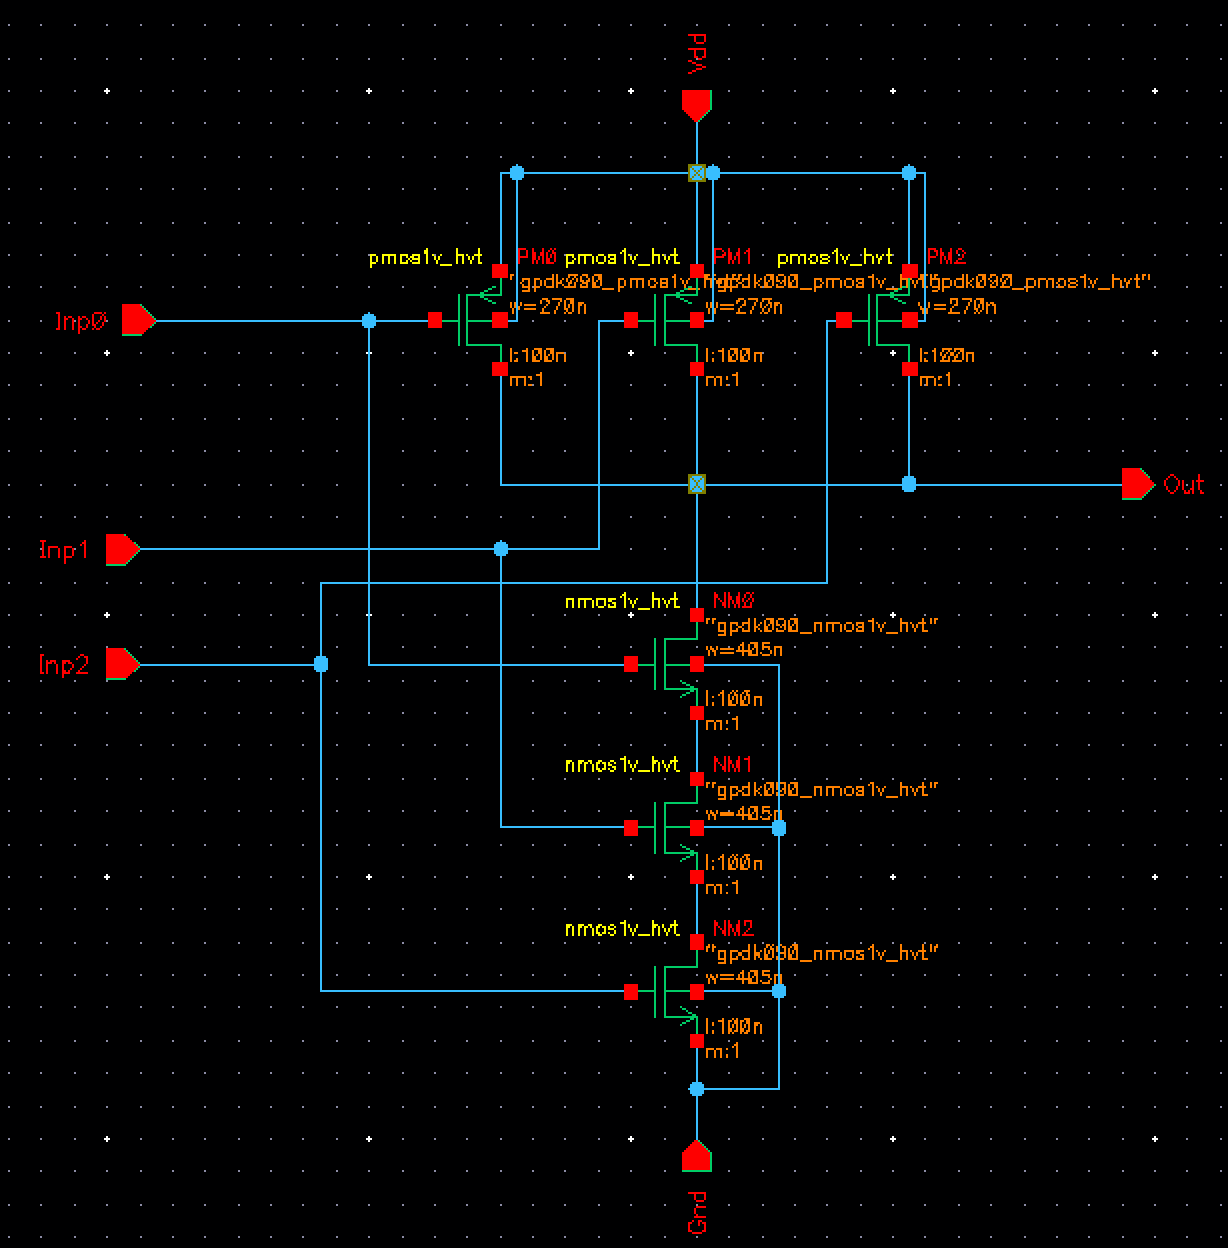
\includegraphics[scale=0.4]{3and.png}
  \\

  3-input xor:\\
  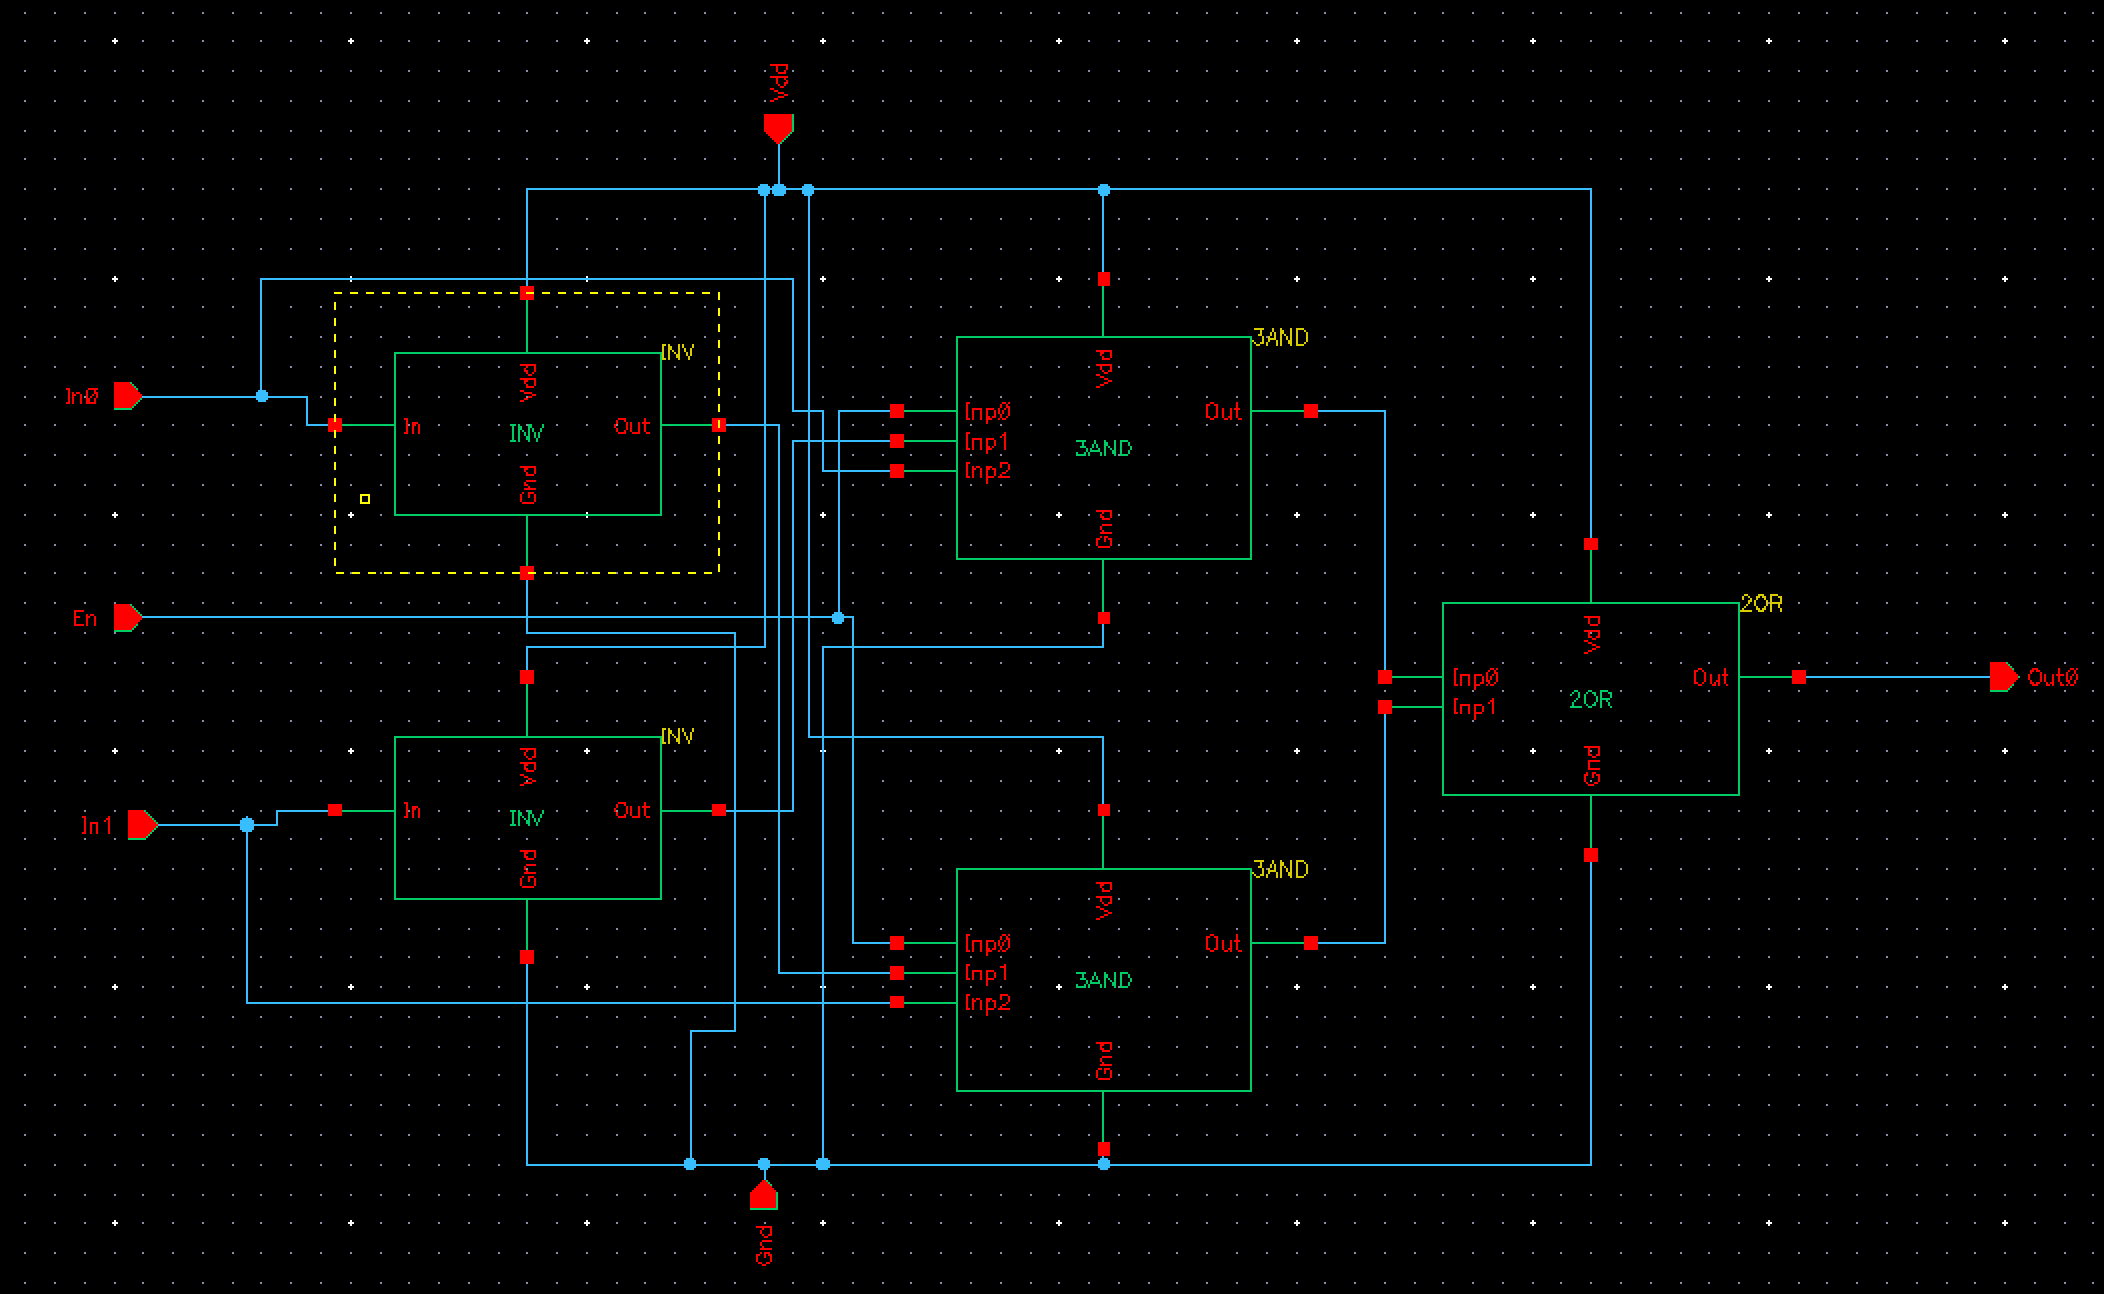
\includegraphics[scale=0.4]{xor.png}
  \\
	
	MUX / DEMUX implementation and uses:
	The primary building blocks for each of these gates were transmission gates, with each 
	T-Gate having a 3$\lambda$ NMOS and a 6$\lambda$ PMOS. These gates primarily served
	as control logic for the circuit (our master schematic heavily relies on DEMUX gates), 
	allowing us to handle multiple input modules and granting us the ability to selectively 
	activate only certain portions of the ALU during any particular OpCode
	in order to minimize power consumption. They also served very crucial roles in allowing us to
	compress the left and right shift modules into one by cleverly mapping the input and easily 
	implement the clear operation. The implementation of these gates are pictured below:
	
  Transmission gate:\\
  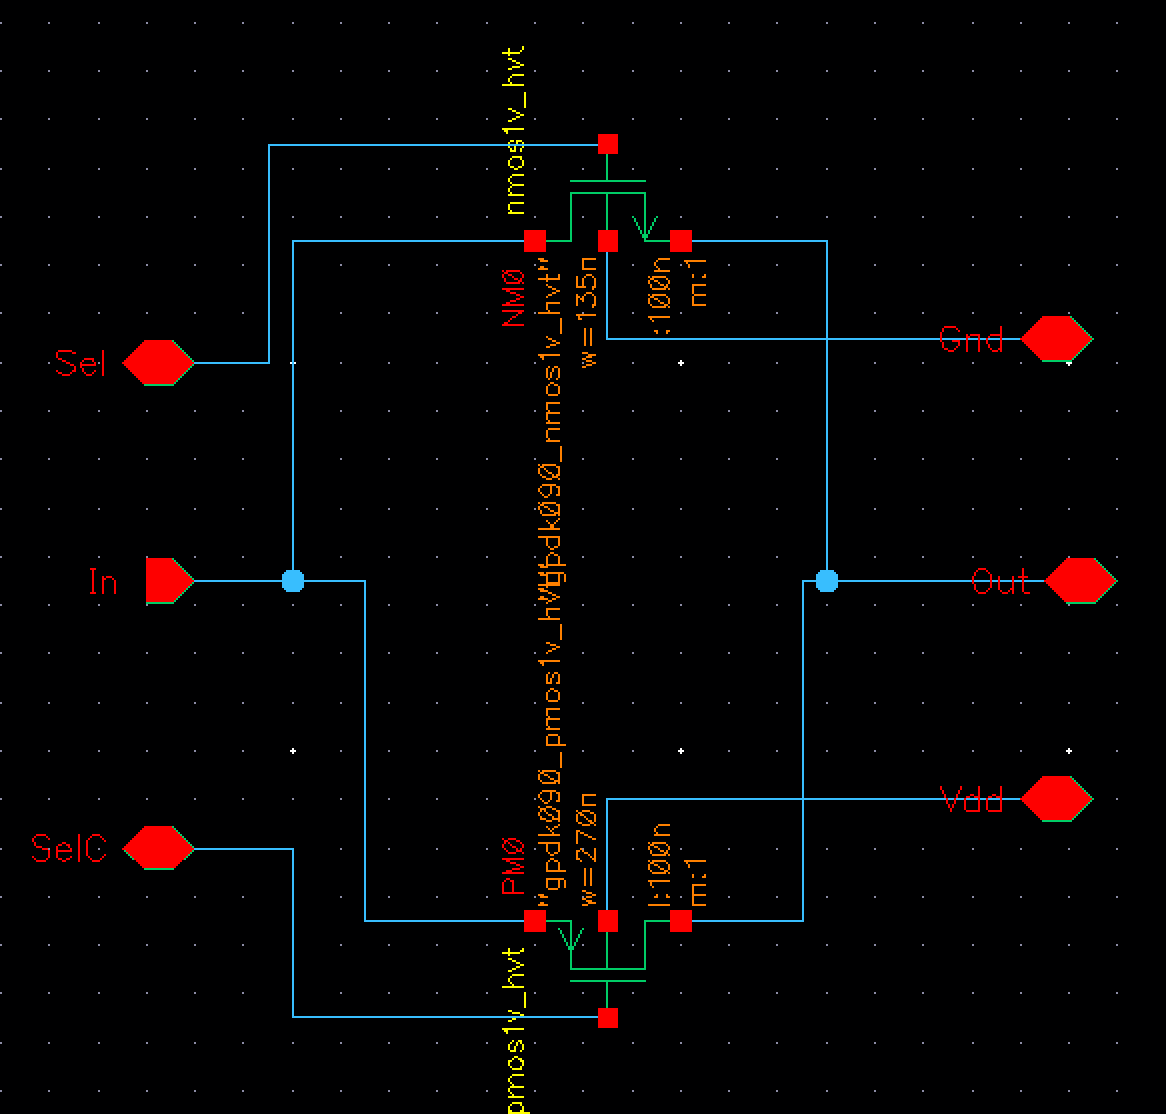
\includegraphics[scale=0.4]{tgate.png}
  \\

  Shifter:\\
  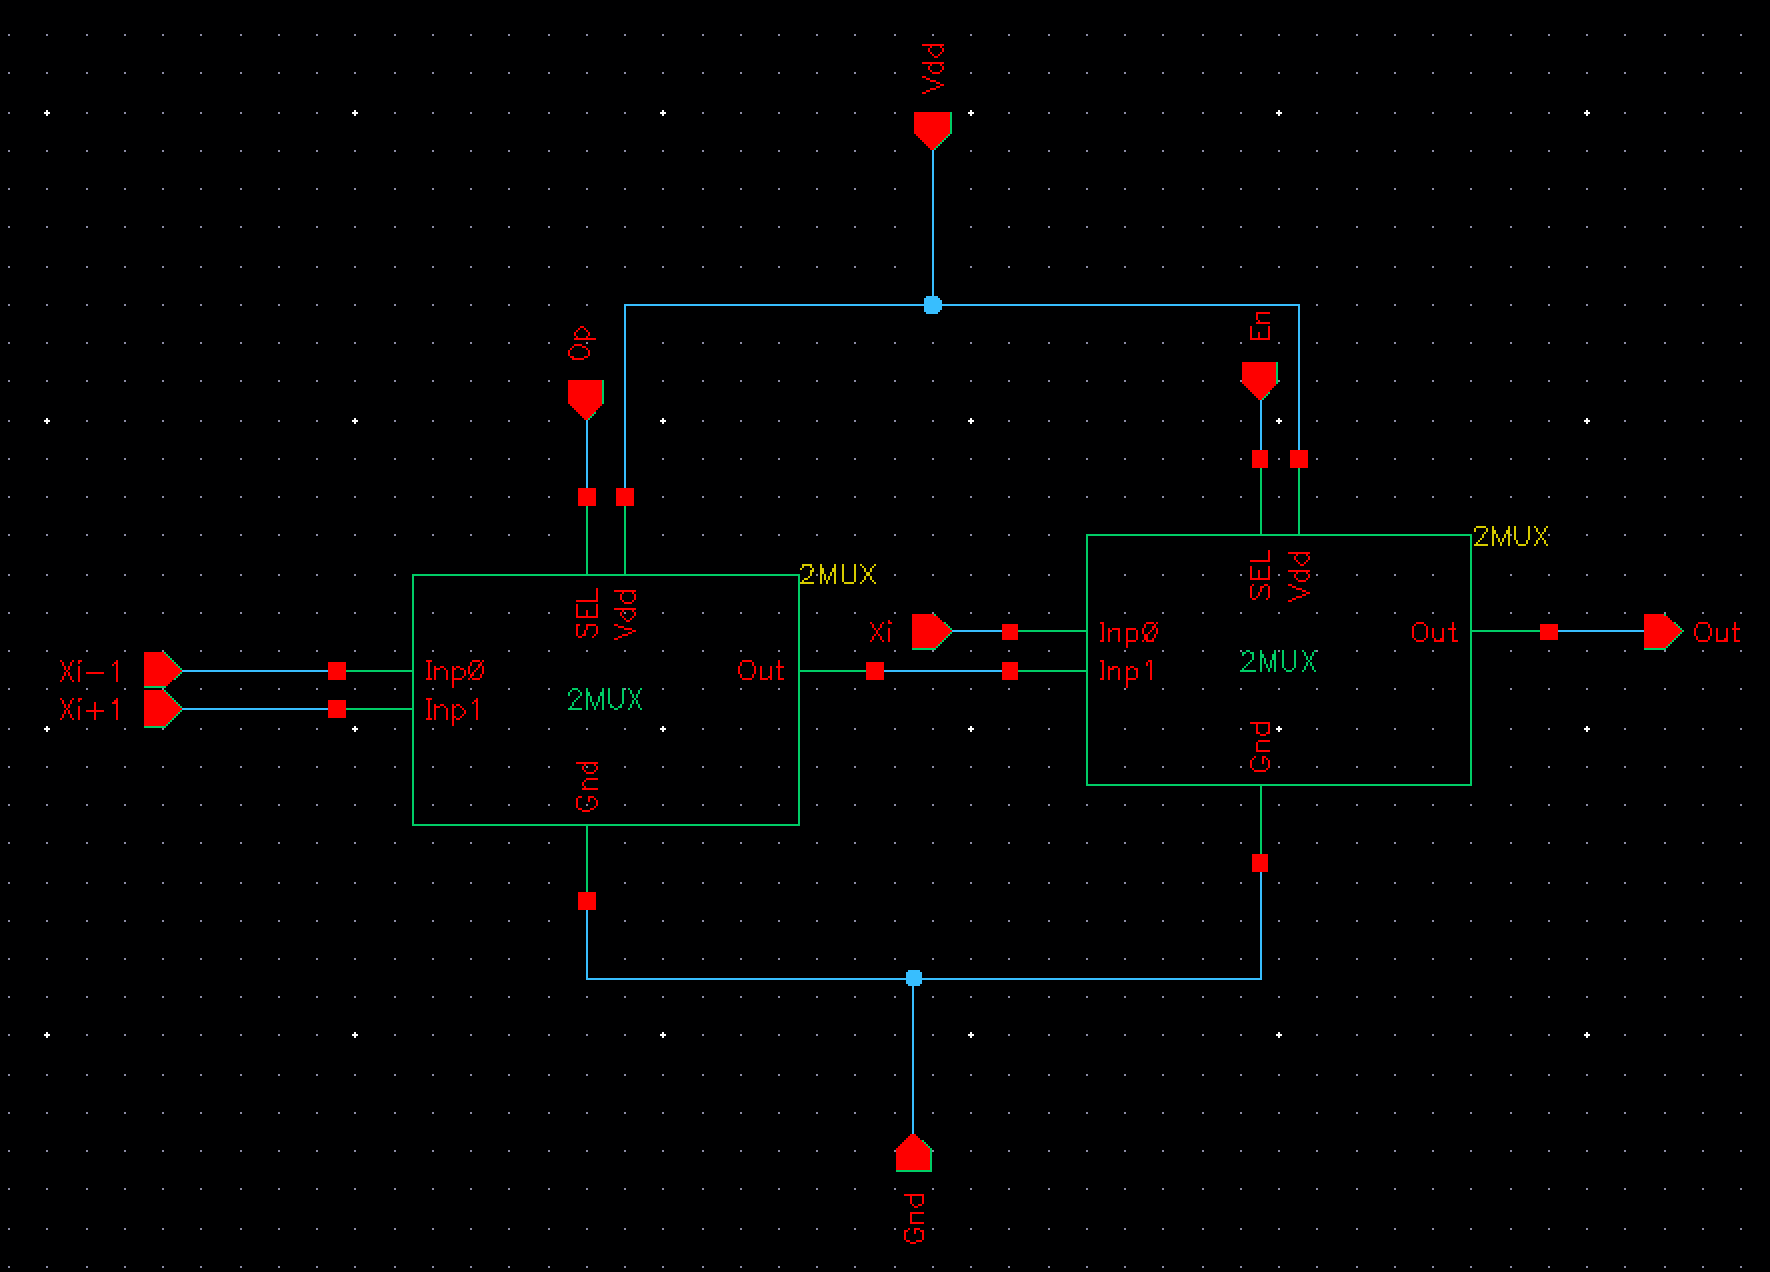
\includegraphics[scale=0.4]{shift.png}
  \\

  Partial Demux:\\
  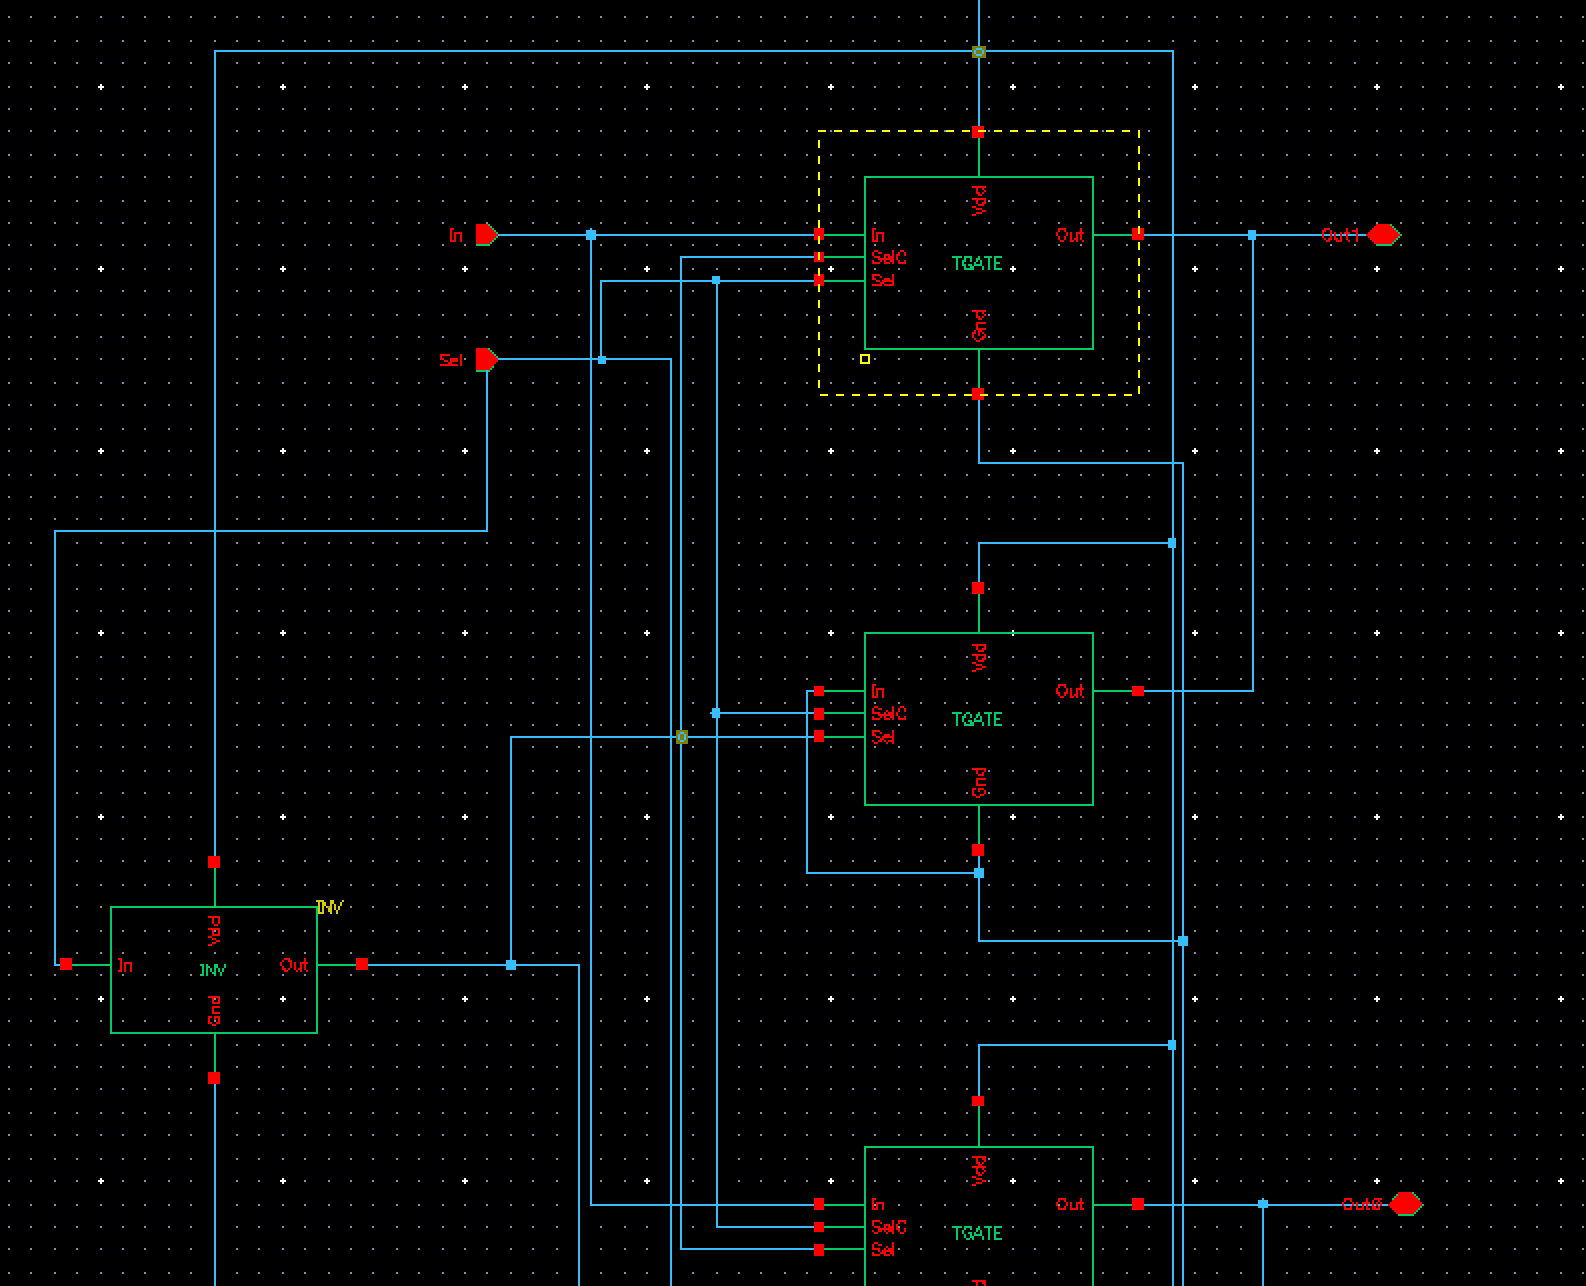
\includegraphics[scale=0.4]{demuxpart.png}
  \\
	
	A final large 8-input MUX was then used to serve as the final channel to the ultimate output 
	bit for the slice. Though each OpCode is 4 bits in length, we managed to come up with an 
	interesting mapping such that only the 3 least significant bits are used:
	
  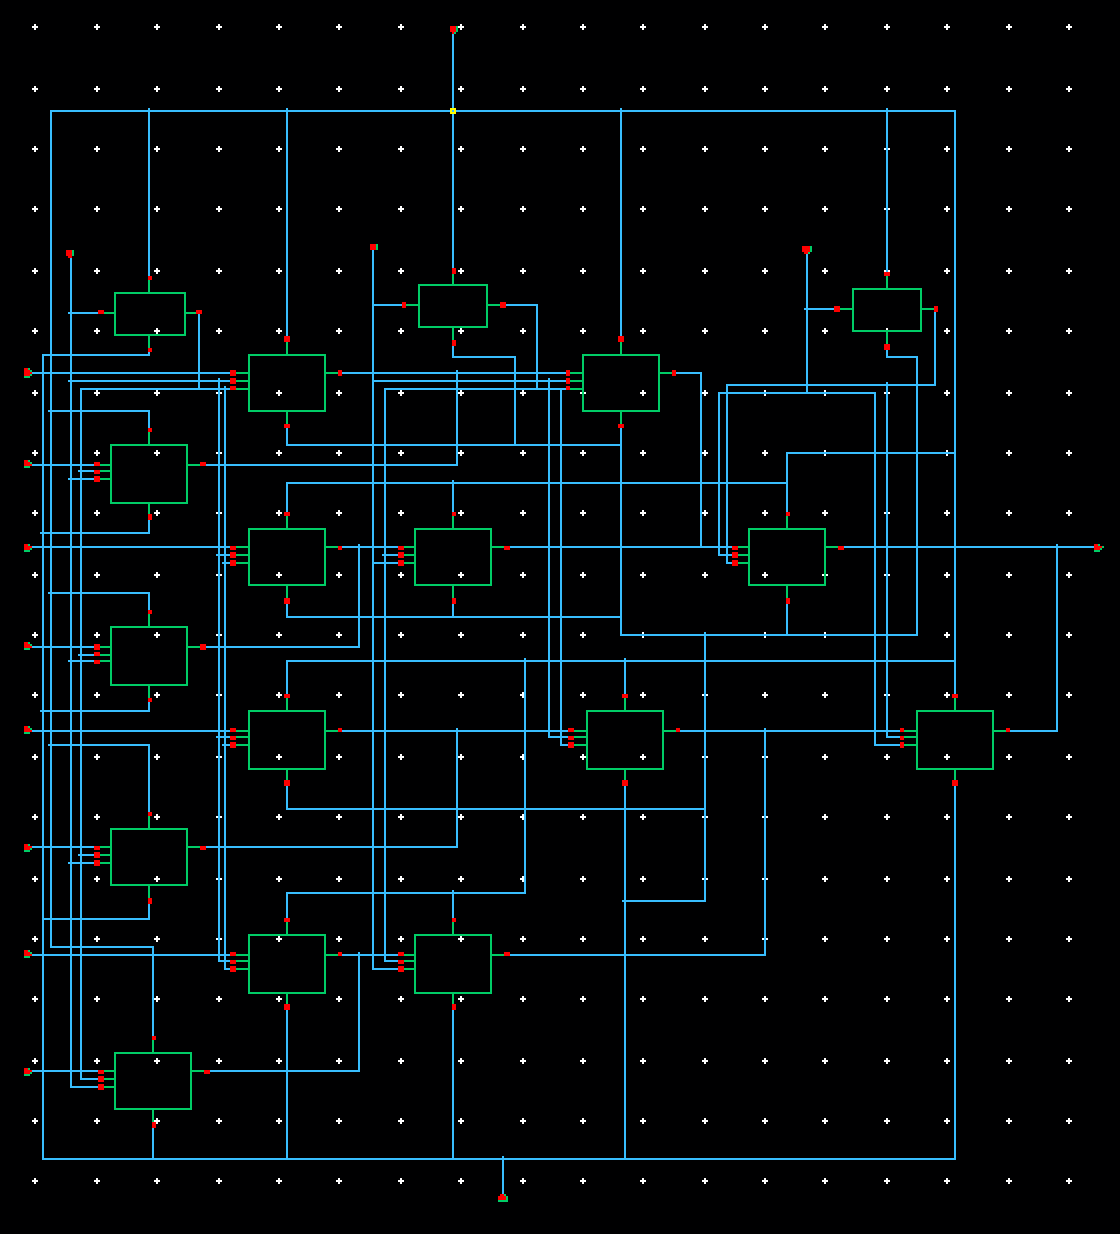
\includegraphics[scale=0.4]{8mux.png}
  \\
	
	Adder implementation:
	We chose to go with a Carry Look-Ahead adder implementation using a combination of AND,
	OR, and XOR gates, as shown below:
	
  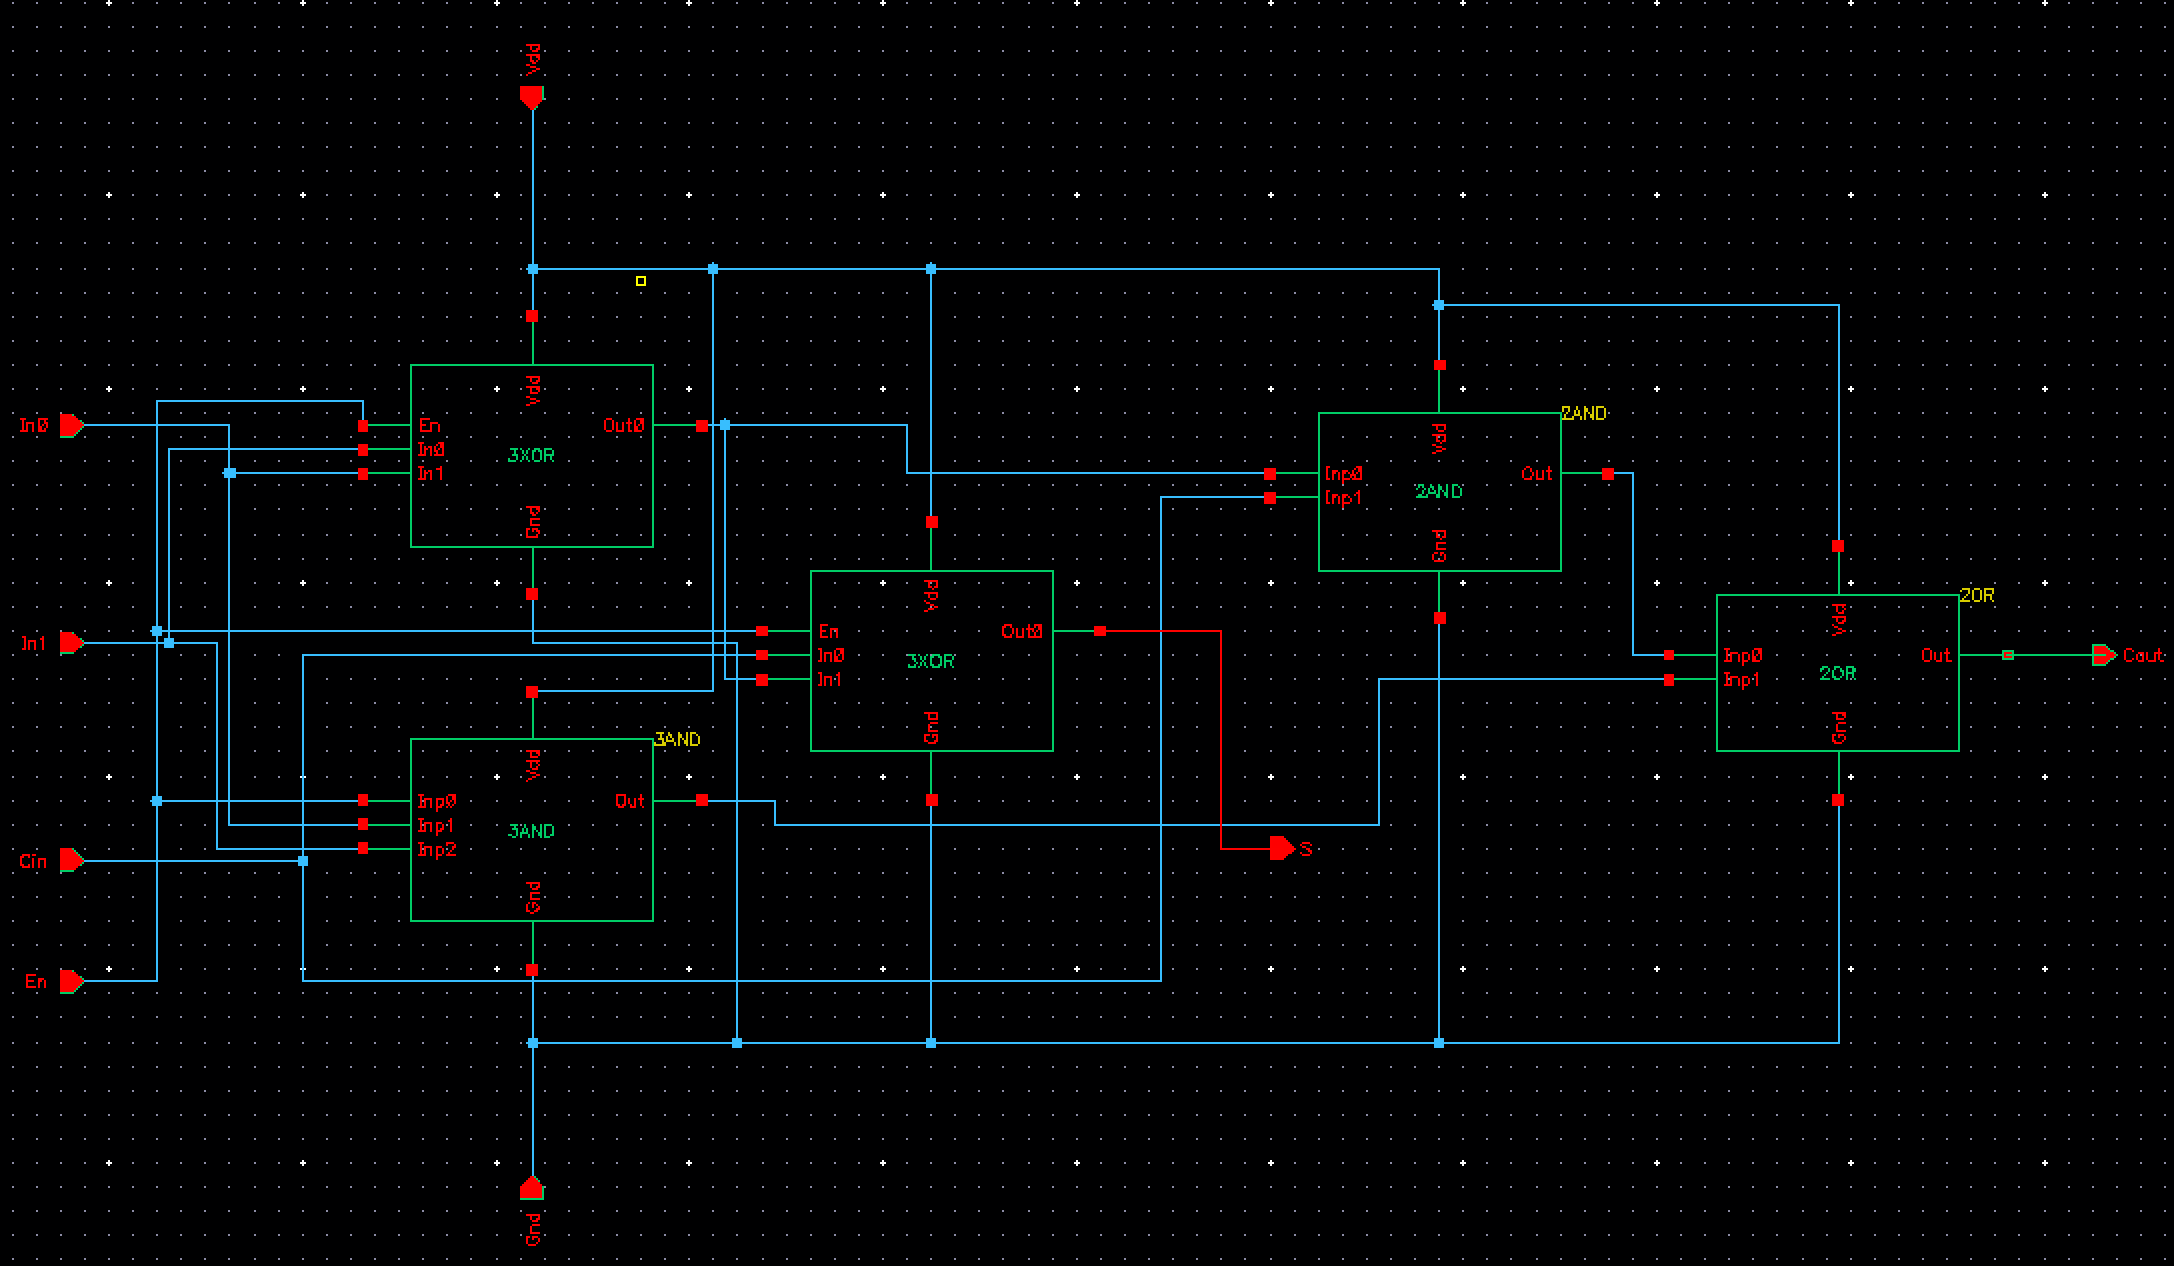
\includegraphics[scale=0.4]{add.png}
  \\

	
	The Look-Ahead implementation would allow for the parallel computation of the Carry-Out and
	Sum quantities, which would allow us to quickly send the carry-out number on the look-ahead
	bus for other bit slices to absorb. In this regard, we would be significantly reducing the delay
	of the adder module and a reasonable amount of power consumption as well. This minimization
	is further supported by the fact that the adder does not even activate unless the enable bit
	is activated (controlled via a combination of DEMUX gates). Future iterations of the project 
	may include changing this implementation, but for now the attempt seemed good enough to
	suffice.
	
	Ending Remarks:
	All components were tested individually for correct functionality before being incorporated 
	into other blocks of the circuit. To test the high level bit slice, we set up a test bench using
	the following setup:
	
  \\
  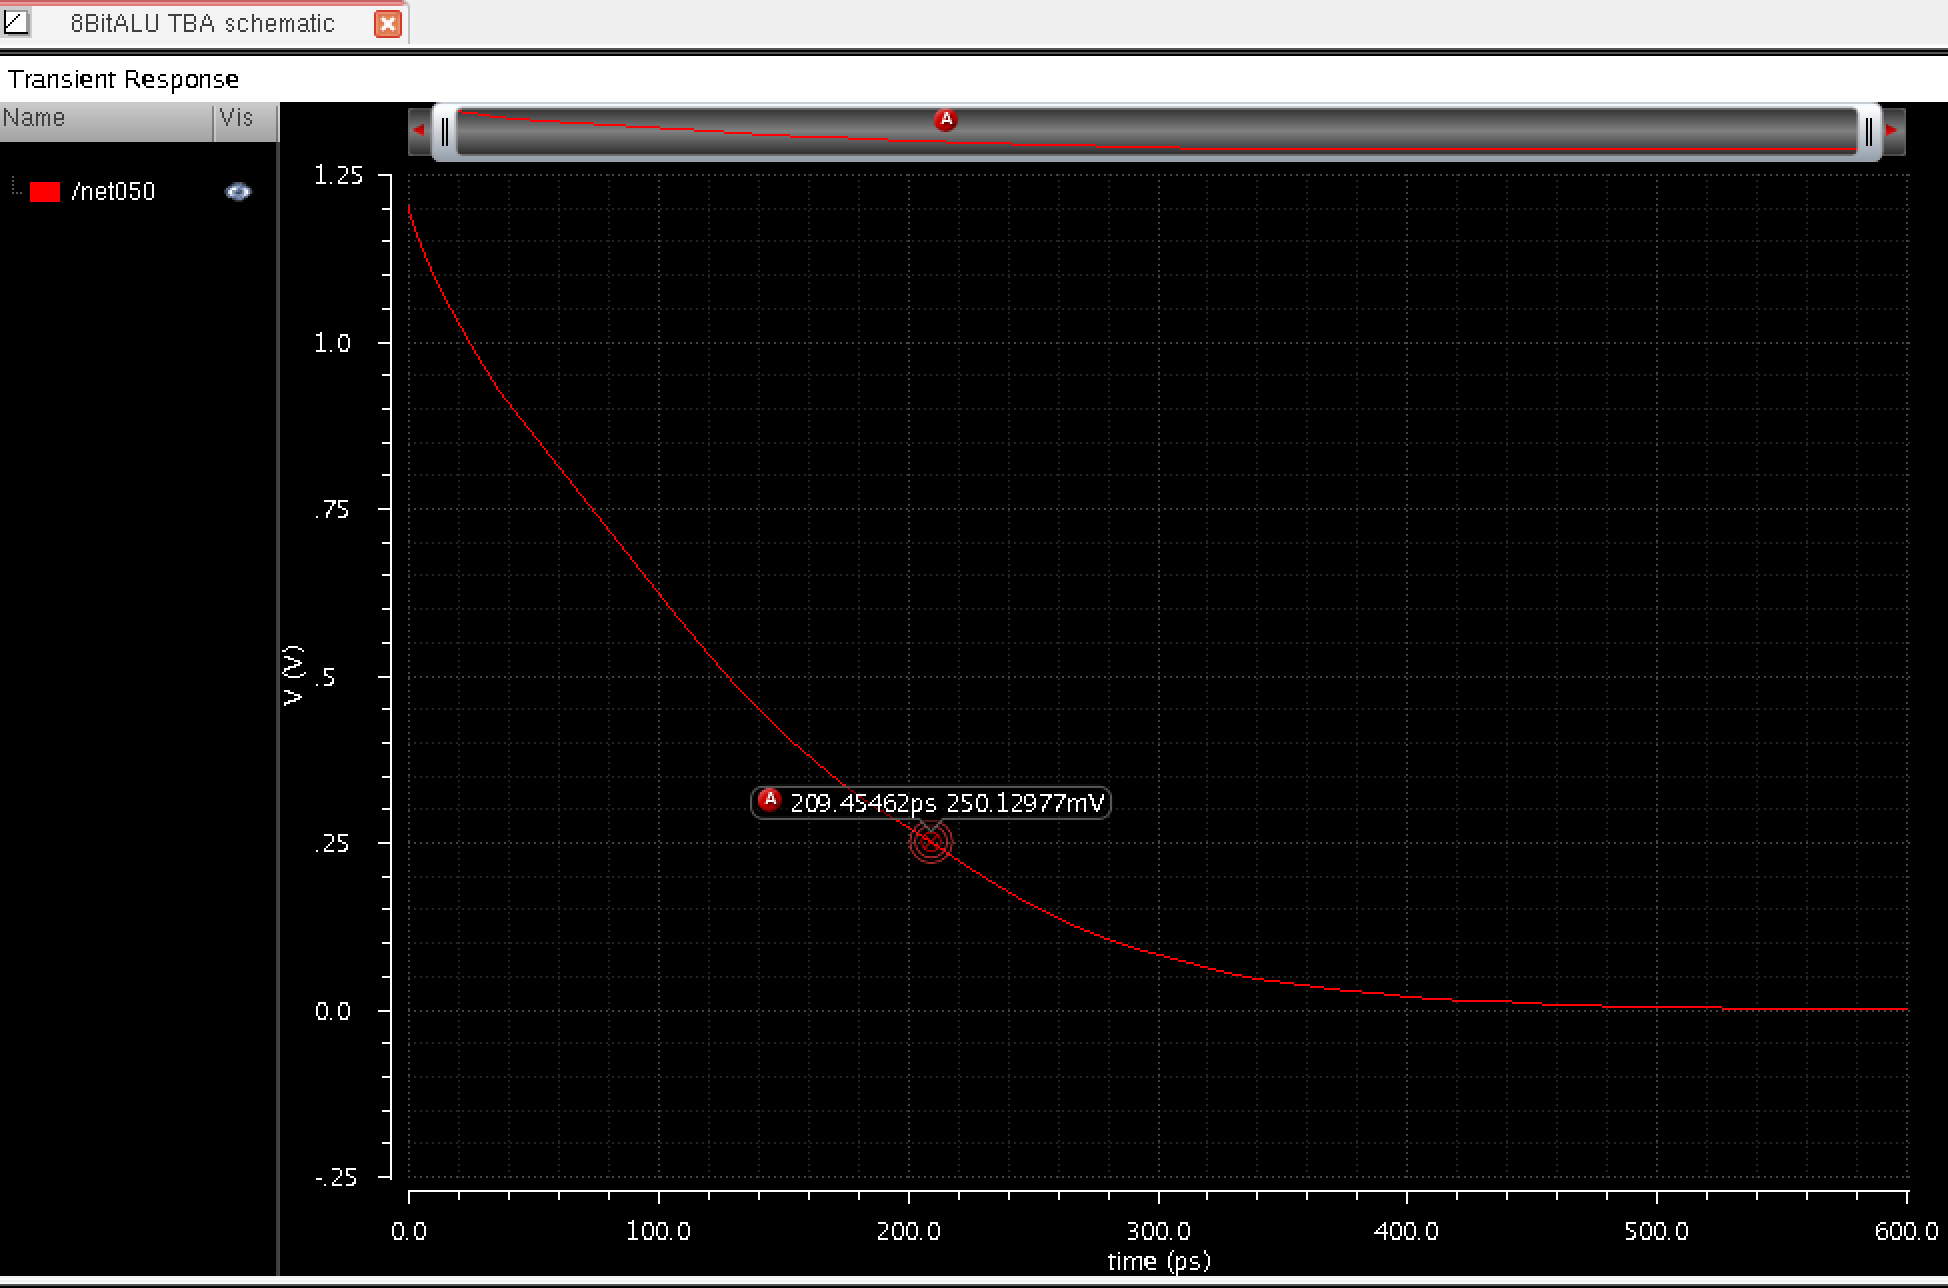
\includegraphics[scale=0.4]{AndDelay.png}
  \\

  This demonstrates the delay from the Bitwise AND path in the ALU. While not the worst delay
  path in the ALU, it does a resonable approximation that of the work that must be done, since
  it travels along the farthest path, alongside the adder instructions. The propagation delay
  here is about 209 ps.
	
	After trying a variety of OpCodes, we found that the slice worked as far as functionality 
	is concerned. For this stage of the project, this was a reasonable testament of our progress
	and hard work.
	
	Next Steps:
	In addition to doing the full transistor layout, we may also decide to revise our designs. Since
	our circuit is modular, this would be reasonably simple to do. We have also not looked into
	one operation in particular - loading X into memory. For this reason, one particular input pin 
	of the 8-input MUX has been left dangling. It will be connected to the loaded bit value of
	X after this block has been implemented. 


\end {document}


